\newcommand{\lstc}[1]{\lstset{language=C,basicstyle=\ttfamily\footnotesize}\lstinline?#1?}

\chapter{Introduction}
\setupuuchapterbib
In this dissertation, we explore multi-language program verification using the \\ SMACK~\cite{smack-cav} software verification toolchain.
%
We begin by adding support for the Rust programming language, then explore adding additional programming languages.
%
Finally, we investigate practical applications of these multi-language additions to SMACK.

\section{Background}
Rust~\cite{rust14} is a new programming language with an emphasis on program safety.
%
Rust statically prevents many memory safety issues through its type system.
%
Some safety issues, such as undefined behavior arising from signed-integer overflow, are checked at runtime.
%
Some features require the use of \textit{unsafe code}, which are regions of code that use operations that could violate memory safety, such as pointer arithmetic.
%
For example, unsafe code blocks may be necessary for writing a heap allocator due to working with memory addresses directly.
%
This code is ideally supposed to expose a safe abstraction around potentially unsafe operations, isolating the unsafe code from the rest of the program.

These latter kinds of safety violations are not detectable by the Rust compiler.
%
However, software verification can be used to check some of these classes of errors.
%
Many memory-safety errors, such as use-after-free or null pointer dereference, can be found automatically by many software verifiers.
%
Integer-overflow errors can similarly be detected.
%
The use of a software verifier has many advantages over using test cases because a software verifier can prove correctness for all inputs.

A final category of safety properties we consider are functional correctness properties.
%
Examples include the following:
\begin{itemize}
    \item Simple properties such as ensuring a function always returns an even result.
    \item Ensuring secret information in an information-flow control implementation is only available to authorized users.
    \item Ensuring equivalence of behavior between a C-language program and a version of that program ported into Rust.
\end{itemize}
%
These properties cannot be checked for correctness by the Rust compiler; however we can apply a formal software verifier to check these properties.

\subsection{SMACK}\label{sec:smackground}

SMACK~\cite{smack-icse,smack-cav,smack-web} is an open source, modular software verification toolchain.
%
The core component of SMACK converts low\--level virtual\--machine intermediate\--representation\\ (LLVM IR) code into Boogie intermediate
verification language~\cite{boogie}.
%
The remainder of the SMACK toolchain handles details such as compiling the
source program into LLVM IR and invoking a Boogie verifier.
%
Its modular nature decouples source language details from verification by
leveraging compiler front-ends to translate programs into the Boogie
intermediate verification language through LLVM IR.
%
% Before we implemented the multi-language extensions described in this chapter,
% SMACK had been predominantly used to verify LLVM IR programs produced by the
% clang C compiler.


\cref{fig:vmcaitoolflow} shows the toolflow of SMACK, which proceeds as
follows:
%
\begin{enumerate}
%
\item SMACK first invokes a compiler on the source program, this is clang for C programs, to compile the input
program, SMACK models, and C standard library models (e.g., strings, pthreads,
math). SMACK models contain various verification primitives (e.g., for
generating nondeterministic values) and the encoding of the memory model for
handling of dynamically allocated memory. All of the models are written in C
since SMACK provides a convenient mechanism for interoperating with the
underlying Boogie code, which we describe below.
%
\item SMACK links together all of the generated LLVM IR files into one LLVM IR
program.
%
\item The core \textsc{llvm2bpl} component of SMACK transforms an LLVM IR
program produced by the previous step into a semantically equivalent Boogie
program.
%
\item Finally, a back-end verifier, such as Corral~\cite{corral}, verifies the
generated Boogie program using an SMT solver, such as Z3~\cite{z3}.
%
\end{enumerate}
%
In this work, we use Corral and Boogie in their bounded verification mode, meaning that it
unrolls loops and recursion up to a certain user-provided bound.


SMACK models verifier primitives and memory models through the use of
\lstc{\_\_SMACK\_code} function. 
%
This C routine takes a formatted string as a parameter, and is declared in the
SMACK header files, but not implemented in any models. 
%
When \textsc{llvm2bpl} comes across a call to this function, instead of
translating the function call, it simply inserts the parameters into the Boogie
code snippet passed as string; this functionality is akin to C's inline
assembly.
%
This allows for Boogie code or ghost variables to be injected into the
translation, giving an easy way to encapsulate routines like \texttt{assume}
which are not normally available in C.
%
It also provides an abstraction that can be used for any primitive or model.


% The SMACK~\cite{smack14} software verifier was originally intended to verify programs written in the C programming language.
% %
% An innovation of SMACK was to use the LLVM~\cite{lattner2004llvm} intermediate representation (LLVM IR), rather than using a direct representation of C programs.
% %
% The reduced complexity of LLVM IR made it easier to build a verifier based on it, because there are fewer instructions to model.

% After the compiler produces LLVM IR code for the C language program, SMACK translates it into the Boogie~\cite{boogie} intermediate verification-language.
% %
% SMACK then uses a Boogie language verifier, such as boogie~\cite{boogie} or corral~\cite{corral}, to perform verification of the translated program.
% %
% The Boogie language verifier translates the program into an SMT-LIB~\cite{smtlib} query to check for assertion violations, and uses an SMT solver, such as Z3~\cite{z3} to verify the program.

\section{Motivation}
We will explore some problems that will help us gauge the need for enhancements for the SMACK verifier, and evaluate the success of these enhancements.

\subsection{Rust in SMACK}
The default backend for the Rust compiler, rustc, uses LLVM to generate machine code.
%
We can capture the LLVM IR produced by rustc to potentially use it in SMACK.
%
SMACK's use of LLVM IR presents the possibility of building a ``universal'' verifier in the sense that it could in theory support every programming language with a compiler targeting LLVM IR.
%
This was only true for the simplest programs, due to incomplete modeling of LLVM by SMACK.
%
SMACK can still serve as a base upon which to build a more universal verifier, and it already models most of the constructs of LLVM.

An additional benefit to using SMACK as a foundation comes from using LLVM IR as a common language to verify programs written in more than one language.
%
For programming languages which can be turned into LLVM IR and have support for calling external C functions, SMACK's features can be integrated into those languages through SMACK's own C library.
%
Programs written in Rust for example can use functions written in C and have them verified together within SMACK.
%
This would not be trivial if SMACK instead translated programs directly from C to Boogie for example.

Finally, SMACK has a developed C library which is optimized for verification.
%
Adding support for a programming language, such as Rust, to SMACK, requires the usage of some of these libraries.
%
These programming languages can inherit the optimizations already done in SMACK's library.
%
This makes it easier to make verifier optimized libraries by leveraging SMACK.


\subsection{Information Flow Control}\label{sec:ifc}
A Rust program we would like to verify is an implementation of an information flow control library for an operating system kernel.
%
Information flow control means that access to resources can only be accessed by users with a minimum authority.
%
Information can also have its authority upgraded, meaning lower authorized users may lose access in the future.
%
In~\cref{lst:rustifc} we can see one such use of a \texttt{SecVec} (secure vector) which can show information flow control is implemented correctly for the \texttt{SecVec} type.

The \texttt{SecVec} type is built on Rust's standard library's dynamically sized array, \text{Vec}.
%
The methods of \texttt{SecVec} are versions of the methods of \texttt{Vec} class's methods with an additional authorization label field.
%
This label controls the authorization level needed to access or modify an index of the underlying vector.
%
The \texttt{SecVec} type therefore aims to add information flow control to the indices of the vector.

In this example, we can verify that flow control is properly implemented for the \texttt{SecVec} type.
%
We begin by creating three variables \texttt{nd1}, \texttt{nd2} and \texttt{nd3}.
%
These variables are constrained so that \texttt{nd1} has at most the same authorization as \texttt{nd3}.
%
The \texttt{nd2} authorization level is constrained to be strictly less than that of \texttt{nd3}.
%
On~\cref{line:lowauthadd}, a secret, \texttt{lsecret}, is added to the secure vector \texttt{s} with the authorization of \texttt{nd1}.
%
Next, on~\cref{line:hiauthadd}, the secret that was added is updated to be \texttt{hsecret}, and its authorization is upgraded to that of \texttt{nd3}.
%
Then, in~\cref{line:lowauthacc}, the an attempt to access the secret is made with the authorization of \texttt{nd2}.
%
This should not lead to an assertion violation because the access should not be authorized.
%
Finally, on~\cref{line:hiauthacc}, an access is attempted with the authorization of \texttt{nd3} and this should succeed, and the assertion in \texttt{check\_label} should pass.
%
If this program can be verified, it would show the correctness of flow control in the \texttt{SecVec} type.

There are several things that need to be added to SMACK in order to verify this program.
%
A Rust-language library needs to be developed which provides the following:
\begin{itemize}
    \item Implementations of \texttt{verifier\_assert} and \texttt{verifier\_assume} in terms of SMACK's \texttt{\_\_VERIFIER\_assert} and \texttt{\_\_VERIFIER\_assume} functions.
    \item Add functions to get nondeterministic values from SMACK's nondeterministic value functions.
    \item And add a Vec class that is amenable to verification within SMACK.
\end{itemize}
%
All of these can be implemented in SMACK for Rust through the use of Rust's foreign function interface which allows Rust to use SMACK's C-language models.
%
With support for these features, SMACK becomes a basic verifier for non-trivial Rust language programs.

\subsection{Generality of Adding Languages to SMACK}
\label{sec:gensmack}
Recently, LLVM has become a popular back-end for many compilers for different languages.
%
These languages include: Rust, Fortran, D, Objective-C, Swift, and Kotlin.
%
Because these languages have back-ends that target LLVM, it should be possible to apply SMACK to LLVM IR generated by their respective compilers.

This is a generalization of adding support for the Rust programming language to \\ SMACK.
%
As with adding support for Rust, simple programs are expected to work in SMACK without many modifications.
%
Like with programs in Rust, programs that use more advanced language or library features may not be immediately supported.
%
This will require improved modeling of LLVM patterns and the development of models of functionality from each language's standard library.

Because of the maturity of the SMACK verifier, unmodeled patterns in LLVM are not anticipated to be the major barrier to adding support for a new language.
%
The modeling effort for LLVM also tests the hypothesis that improvement to SMACK's LLVM support for one language benefits all languages added to SMACK.
%
Conversely, the modeling effort for a language's standard library may be much more significant, similar to adding a verifier friendly version of the \texttt{Vec} type for Rust.

SMACK is oriented around verifying individual programs, such as a single C or a single Rust program.
%
This is despite SMACK automatically linking the SMACK C-language library for verification of programs written in non-C languages.
%
SMACK can be extended to automatically handle programs written in multiple languages.
%
For example, we could have versions of a function written in Rust, Swift and C, and verify the equivalence of behavior between them.
%
This is shown in~\cref{fig:factrsc}.

These extensions would move SMACK closer to being a universal verifier for programming languages that can target LLVM.
%
The improvements to SMACK's modeling of LLVM are beneficial for all languages which it supports.
%
And this would help deliver on SMACK's promise of being a mult- and cross-language verifier.

\subsection{Equivalence Checking of Source-Level Ports}
New programming languages, such as Rust, may not have native-language version of many libraries that are standard or ubiquitous in more mature programming languages.
%
It is possible to use a foreign function interface to use existing libraries, often written in C, to provide the missing functionality.
%
This may not always be the best option for implementing these libraries.
%
For example, foreign language code may not be as able to be optimized, e.g., due to a lack of inlining, and may not be ideal for debugging.

Specific to Rust, calls to foreign functions are considered to be unsafe.
%
This causes the entirety of this code to be considered unsafe, when it may not have any unsafe operations if it were written in Rust.
%
Limiting, or eliminating unsafe code is desirable in Rust programs as it reduces the potential problems that may arise from unsafe code.

These libraries can be ported from the source language to the new programming language.
%
For example, a math library written in C, such as \texttt{musl}~\cite{musl} libm, can be ported to Rust, almost statement by statement.
%
A source level port such as this helps to overcome issues with optimization and reduces the presence of unsafe code.
%
However, this may not produce a correct version of the function in Rust.

Consider the \texttt{musl} implementation of the \texttt{acosf} function in~\cref{fig:acosfintro}.
%
In~\cref{fig:acosfintro}, we can see a port of the prior C function as ported into Rust.
%
While there are no safety properties to check, such as memory-safety, integer-overflow, the two programs should have the same behavior for the port to be considered correct.


This program uses both floating-point and bit-wise operations.
%
These necessitate the use of the SMT floating-point and bit-vector operations.
%
Programs tend to be slower to verify due to the difficulty of these theories.
%
However, it may be possible to help SMACK take advantage of the similarity of the two programs.
%
In~\cref{fig:acosfintro}, it can be seen that line-by-line, the two programs are doing very similar things, in the same order.
%
Because of this, it may be possible to extend SMACK to provide functionality to help match expressions between the programs when checking them for equivalence.

\section{Contributions}
In the work in \Cref{cha2}, we made the following extensions to SMACK:
\begin{itemize}
    \item We extended the \texttt{llvm2bpl} component to support new LLVM instructions used by the Rust compiler that were not modeled.
    \item We built a SMACK library which provides models for verification primitives and verification friendly implementations of Rust standard library functionality, such as the \texttt{Vec} class.
    \item We applied SMACK to verify an implementation of the IFC system described in \cref{sec:ifc}.
    \item We performed primitive multi-language verification.
\end{itemize}

In \Cref{cha3}, we made the following contributions:
\begin{itemize}
    \item We applied the techniques from \Cref{cha2} to add support for several multiple programming languages to SMACK. These include Swift, Objective-C and Fortran.
    \item We made extensions to \texttt{llvm2bpl} to support new constructs in LLVM arising from the new programming languages.
    \item We modified SMACK to automate the process of linking and combining programs from different programming languages.
    \item We performed an equivalence check between functions written in C, Rust and Fortran programs.
    \item We performed equivalence checking of a half-precision library written in Rust and C and identified bugs.
\end{itemize}

Finally, in \Cref{chap4} we made the following contributions:
\begin{itemize}
    \item We applied SMACK to a Rust-language port of the \texttt{musl} math library.
    \item We developed extensions to SMACK to help with scalability issues.
    \item We found some bugs in the Rust library, including one that could not be found via testing.
\end{itemize}

\section{Dissertation Statement}
\newcommand{\thesisstmt}{Software verifiers that operate on a common intermediate language can be effectively extended to support new programming languages through a general approach that enables multi-language and cross-language verification.}

\thesisstmt

%\marek{The flexibility of software verifiers built on a common intermediate language allows for lower-effort integration of new languages, and provides for a general framework for multi-language and cross-language verification that is practical for validating the correctness properties between languages.
%}


\bibliographystyle{plain}
\bibliography{refs}
\newpage
\begin{figure}[tbh]
	\centering
	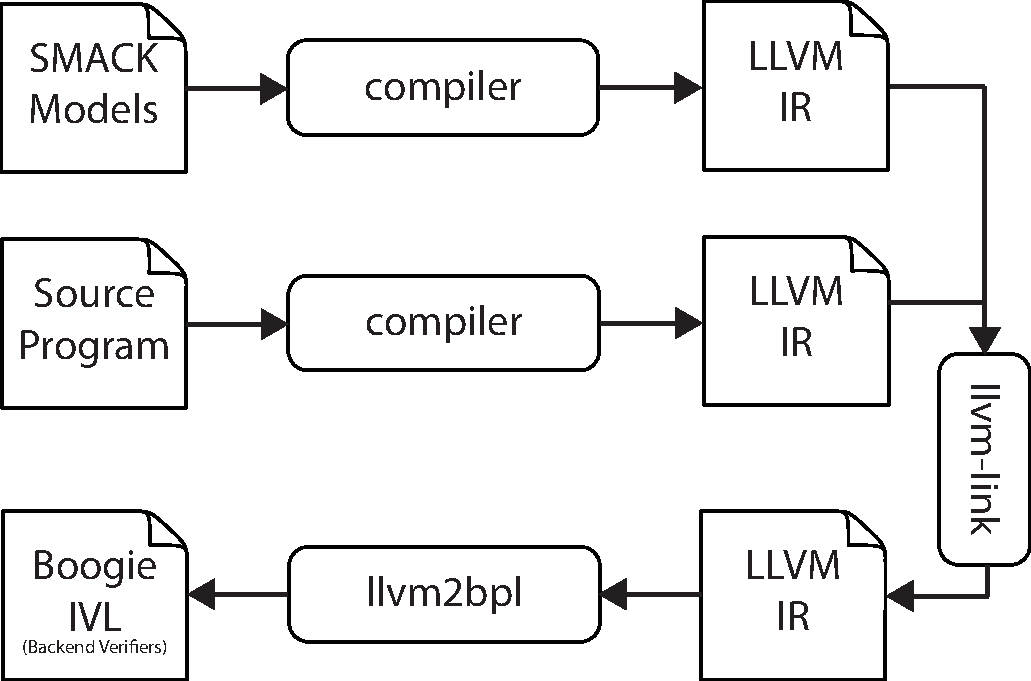
\includegraphics[width=\textwidth]{chap1/fig/SMACKIntro.pdf}
	\caption{Toolflow of SMACK.}
	\label{fig:vmcaitoolflow}
\end{figure}

%%%%%%%%%%%%%%%%%%%%%%%%%%%%%%%%%%%%%%%%%%%%%%%%%%%%%%%%%%%%%%%%%%%%%%%%%%%%%%%%%%%%%%%%%%

\begin{figure}[tbh]
%\begin{lstlisting}[language=Rust, label={lst:rustifc}, caption=Information flow control example in Rust., style=boxed, escapechar=`, float=tbh, captionpos=b, basicstyle=\small=]
\begin{lstlisting}[language=Rust, style=boxed, escapechar=`, captionpos=b, basicstyle=\small=]
fn check_label(x: SVec, l: Label) {
    verifier_assert!(x.l == l);
}

fn main() {
    let nd1: u64 = 5.verifier_nondet();
    let nd2: u64 = 5.verifier_nondet();
    let nd3: u64 = 6.verifier_nondet();

    // Ensure nd1 and nd3 have authorization greater than 4.
    // Ensure nd1 have at most the authorization of nd3.
    // Ensure nd2 have lower authorization than nd3.
    verifier_assume!(nd1 > 4 && nd3 > 4);
    verifier_assume!(nd1 <= nd3);
    verifier_assume!(nd2 < nd3);

    let mut s: SecVec = SecVec::new();
    let lsecret: SVec = svec![1,2,3 => nd1];
    let hsecret: SVec = svec![4,5,6 => nd3];

    // Add lsecret with nd1 authority.
    s.push(lsecret, nd1);`\label{line:lowauthadd}`
    // Update secret to hsecret with nd3 authority.
    s.update(0, hsecret, nd3);`\label{line:hiauthadd}`

    // Reading secrets with low authority
    match s.get(0, nd2) {`\label{line:lowauthacc}`
        None    => {},
        Some(sec) => {
            // Unreachable
            verifier_assert!(false);
            let label1 = sec;
            check_label(label1, nd2);
        }
    }

    // Reading secrets with high authority
    match s.get(0, nd3) {`\label{line:hiauthacc}`
        None      => {},
        Some(sec) => {
            let label2 = sec;
            // Check passes
            check_label(label2, nd3);
        }
    }
}
\end{lstlisting}
\caption{Information flow control example in Rust.}
\label{lst:rustifc}
\end{figure}

%%%%%%%%%%%%%%%%%%%%%%%%%%%%%%%%%%%%%%%%%%%%%%%%%%%%%%%%%%%%%%%%%%%%%%%%%%%%%%%%%%%%%%%%%%

\begin{figure}[tbh]
\begin{minipage}{.33\textwidth}
%\begin{lstlisting}[language=Rust, caption={Implementation of the factorial function in Rust.}, style=boxed, escapechar=`, captionpos=b, float=tbh, label=lst:factrs]
\begin{lstlisting}[language=Rust, style=boxed, escapechar=`]
fn fact(n: u32)
  -> u32
{
  let mut res = 1;
  for i in 1..=n
  {
    res *= i;
  }
  return res;
}
\end{lstlisting}
\end{minipage}
%
\begin{minipage}{.33\textwidth}
%\begin{lstlisting}[language=C, caption={Implementation of the factorial function in Swift.}, style=boxed, escapechar=`, captionpos=b, float=tbh,label=lst:factswift]
\begin{lstlisting}[language=C, style=boxed, escapechar=`]
func fact(n:UInt32)
  -> UInt32
{
  var result = 1
  for i in 1...n
  {
    result *= i
  }
  return result
}
\end{lstlisting}
\end{minipage}
%
\begin{minipage}{.33\textwidth}
%\begin{lstlisting}[language=C, caption={Implementation of the factorial function in C.}, style=boxed, escapechar=`, captionpos=b, float=tbh,label=lst:factc]
\begin{lstlisting}[language=C, style=boxed, escapechar=`]
uint32_t
fact(uint32_t n)
{
  uint32_t res = 1;
  for (uint32_t i = 1;
       i <= n; ++i) {
    res *= i;
  }
  return res;
}
\end{lstlisting}
\end{minipage}
\caption{Implementations of the factorial function in Rust (left), Swift (center) and C (right).}
\label{fig:factrsc}
\end{figure}

%%%%%%%%%%%%%%%%%%%%%%%%%%%%%%%%%%%%%%%%%%%%%%%%%%%%%%%%%%%%%%%%%%%%%%%%%%%%%%%%%%%%%%%%%%

\begin{figure}[tbh]
\begin{minipage}{.5\textwidth}
%\begin{lstlisting}[language=C, label={lst:muslacosfintro}, caption=Source of acosf.c from \texttt{musl} libm, style=boxed, escapechar=`, basicstyle=\small, float=tbh, captionpos=b]
\begin{lstlisting}[language=C, style=boxed, escapechar=`, basicstyle=\small]
float acosf(float x) {
  float z,w,s,c,df;

  uint32_t hx,ix;
  GET_FLOAT(hx, x);
  ix = hx & 0x7fffffff;
  /* |x| >= 1 or nan */
  if (ix >= 0x3f800000) {
    if (ix == 0x3f800000) {
      if (hx >> 31)
        return 2*pio2_hi +
               0x1p-120f;

      return 0;
    }
    return 0/(x-x);
  }
  /* |x| < 0.5 */
  if (ix < 0x3f000000) {
    /*|x|<2**-26*/
    if (ix<=0x32800000)
      return pio2_hi + 0x1p-120f;

    return pio2_hi - 
           (x-(pio2_lo-x*R(x*x)));
  }
  /* x < -0.5 */
  if (hx >> 31) {
    z = (1+x)*0.5f;
    s = sqrtf(z);
    w = R(z)*s-pio2_lo;
    return 2*(pio2_hi - (s+w));
  }
  /* x > 0.5 */
  z = (1-x)*0.5f;
  s = sqrtf(z);
  GET_FLOAT(hx,s);
  SET_FLOAT(df,hx&0xfffff000);

  c = (z-df*df)/(s+df);
  w = R(z)*s+c;
  return 2*(df+w);
}
\end{lstlisting}
\end{minipage}
%
\begin{minipage}{.5\textwidth}
%\begin{lstlisting}[language=Rust, label={lst:rustacosfintro}, caption=Source of acosf.rs from Rust libm, style=boxed, escapechar=`, basicstyle=\small, captionpos=b, float=tbh]
\begin{lstlisting}[language=Rust, style=boxed, escapechar=`, basicstyle=\small]
fn acosf(x: f32) -> f32 {
  let x1p_120 =
    f32::from_bits(0x03800000);
  let z:f32;let w:f32;let s:f32;
  let mut hx = x.to_bits();
  let ix = hx & 0x7fffffff;
  /* |x| >= 1 or nan */
  if ix >= 0x3f800000 {
    if ix == 0x3f800000 {
      if (hx >> 31) != 0 {
        return 2. * PIO2_HI +
               x1p_120;
      }
      return 0.;
    }
    return 0. / (x - x);
  }
  /* |x| < 0.5 */
  if ix < 0x3f000000 {
    if ix <= 0x32800000 {
      /* |x| < 2**-26 */
      return PIO2_HI + x1p_120;
    }
    return PIO2_HI -
           (x-(PIO2_LO-x*r(x*x)));
  }
  /* x < -0.5 */
  if (hx >> 31) != 0 {
    z = (1. + x) * 0.5;
    s = sqrtf(z);
    w = r(z) * s - PIO2_LO;
    return 2.*(PIO2_HI - (s + w));
  }
  /* x > 0.5 */
  z = (1. - x) * 0.5;
  s = sqrtf(z);
  hx = s.to_bits();
  let df =
    f32::from_bits(hx&0xfffff000);
  let c = (z-df*df)/(s+df);
  w = r(z) * s + c;
  2. * (df + w)
}
\end{lstlisting}
\end{minipage}
\caption{Implementations of the \texttt{acosf} function in \texttt{musl} libm (left) and Rust libm (right).}
\label{fig:acosfintro}
\end{figure}

% \begin{figure}[tbh]
% 	\centering
% 	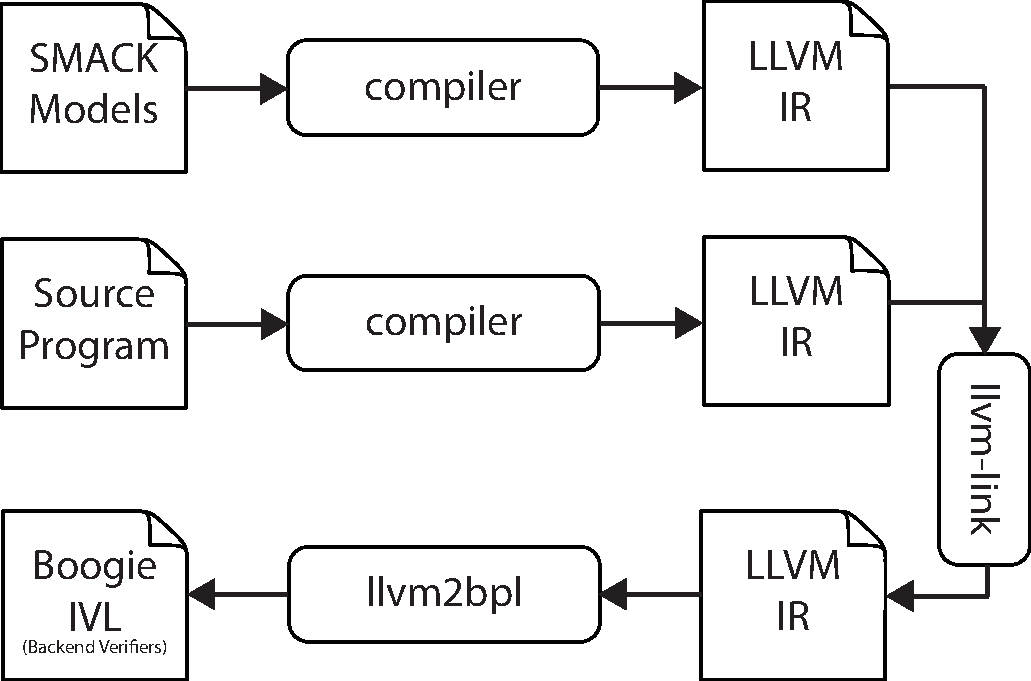
\includegraphics[width=\textwidth]{chap1/fig/SMACKIntro.pdf}
% 	\caption{Toolflow of SMACK.}
% 	\label{fig:vmcaitoolflow}
% \end{figure}

% \begin{lstlisting}[language=Rust, label={lst:rustifc}, caption=Information flow control example in Rust, style=boxed, escapechar=`, float=tbh, captionpos=b, basicstyle=\small=]
% fn check_label(x: SVec, l: Label) {
%     verifier_assert!(x.l == l);
% }

% fn main() {
%     let nd1: u64 = 5.verifier_nondet();
%     let nd2: u64 = 5.verifier_nondet();
%     let nd3: u64 = 6.verifier_nondet();

%     // Ensure nd1 and nd3 have authorization greater than 4.
%     // Ensure nd1 have at most the authorization of nd3.
%     // Ensure nd2 have lower authorization than nd3.
%     verifier_assume!(nd1 > 4 && nd3 > 4);
%     verifier_assume!(nd1 <= nd3);
%     verifier_assume!(nd2 < nd3);

%     let mut s: SecVec = SecVec::new();
%     let lsecret: SVec = svec![1,2,3 => nd1];
%     let hsecret: SVec = svec![4,5,6 => nd3];

%     // Add lsecret with nd1 authority.
%     s.push(lsecret, nd1);`\label{line:lowauthadd}`
%     // Update secret to hsecret with nd3 authority.
%     s.update(0, hsecret, nd3);`\label{line:hiauthadd}`

%     // Reading secrets with low authority
%     match s.get(0, nd2) {`\label{line:lowauthacc}`
%         None    => {},
%         Some(sec) => {
%             // Unreachable
%             verifier_assert!(false);
%             let label1 = sec;
%             check_label(label1, nd2);
%         }
%     }

%     // Reading secrets with high authority
%     match s.get(0, nd3) {`\label{line:hiauthacc}`
%         None      => {},
%         Some(sec) => {
%             let label2 = sec;
%             // Check passes
%             check_label(label2, nd3);
%         }
%     }
% }
% \end{lstlisting}

% \begin{lstlisting}[language=Rust, caption={Implementation of the factorial function in Rust.}, style=boxed, escapechar=`, captionpos=b, float=tbh, label=lst:factrs]
% fn fact(n: u32) -> u32 {
%   let mut res = 1;
%   for i in 1..=n {
%     res *= i;
%   }
%   return res;
% }
% \end{lstlisting}

% \begin{lstlisting}[language=C, caption={Implementation of the factorial function in Swift.}, style=boxed, escapechar=`, captionpos=b, float=tbh,label=lst:factswift]
% func fact(n:UInt32) -> UInt32 {
%   var result = 1
%   for i in 1...n {
%     result *= i
%   }
%   return result
% }
% \end{lstlisting}

% \begin{lstlisting}[language=C, caption={Implementation of the factorial function in C.}, style=boxed, escapechar=`, captionpos=b, float=tbh,label=lst:factc]
% uint32_t fact(uint32_t n) {
%   uint32_t res = 1;
%   for (uint32_t i = 1;
%        i <= n; ++i) {
%     res *= i;
%   }
%   return res;
% }
% \end{lstlisting}


% % \begin{figure}[tbh]
% % \begin{minipage}{.5\textwidth}
% \begin{lstlisting}[language=C, label={lst:muslacosfintro}, caption=Source of acosf.c from musl libm, style=boxed, escapechar=`, basicstyle=\small, float=tbh, captionpos=b]
% float acosf(float x) {
%   float z,w,s,c,df;

%   uint32_t hx,ix;
%   GET_FLOAT(hx, x);
%   ix = hx & 0x7fffffff;
%   /* |x| >= 1 or nan */
%   if (ix >= 0x3f800000) {
%     if (ix == 0x3f800000) {
%       if (hx >> 31)
%         return 2*pio2_hi +
%                0x1p-120f;

%       return 0;
%     }
%     return 0/(x-x);
%   }
%   /* |x| < 0.5 */
%   if (ix < 0x3f000000) {
%     /*|x|<2**-26*/
%     if (ix<=0x32800000)
%       return pio2_hi + 0x1p-120f;

%     return pio2_hi - 
%            (x-(pio2_lo-x*R(x*x)));
%   }
%   /* x < -0.5 */
%   if (hx >> 31) {
%     z = (1+x)*0.5f;
%     s = sqrtf(z);
%     w = R(z)*s-pio2_lo;
%     return 2*(pio2_hi - (s+w));
%   }
%   /* x > 0.5 */
%   z = (1-x)*0.5f;
%   s = sqrtf(z);
%   GET_FLOAT(hx,s);
%   SET_FLOAT(df,hx&0xfffff000);

%   c = (z-df*df)/(s+df);
%   w = R(z)*s+c;
%   return 2*(df+w);
% }
% \end{lstlisting}

% \begin{lstlisting}[language=Rust, label={lst:rustacosfintro}, caption=Source of acosf.rs from Rust libm, style=boxed, escapechar=`, basicstyle=\small, captionpos=b, float=tbh]
% fn acosf(x: f32) -> f32 {
%   let x1p_120 =
%     f32::from_bits(0x03800000);
%   let z:f32;let w:f32;let s:f32;
%   let mut hx = x.to_bits();
%   let ix = hx & 0x7fffffff;
%   /* |x| >= 1 or nan */
%   if ix >= 0x3f800000 {
%     if ix == 0x3f800000 {
%       if (hx >> 31) != 0 {
%         return 2. * PIO2_HI +
%                x1p_120;
%       }
%       return 0.;
%     }
%     return 0. / (x - x);
%   }
%   /* |x| < 0.5 */
%   if ix < 0x3f000000 {
%     if ix <= 0x32800000 {
%       /* |x| < 2**-26 */
%       return PIO2_HI + x1p_120;
%     }
%     return PIO2_HI -
%            (x-(PIO2_LO-x*r(x*x)));
%   }
%   /* x < -0.5 */
%   if (hx >> 31) != 0 {
%     z = (1. + x) * 0.5;
%     s = sqrtf(z);
%     w = r(z) * s - PIO2_LO;
%     return 2.*(PIO2_HI - (s + w));
%   }
%   /* x > 0.5 */
%   z = (1. - x) * 0.5;
%   s = sqrtf(z);
%   hx = s.to_bits();
%   let df =
%     f32::from_bits(hx&0xfffff000);
%   let c = (z-df*df)/(s+df);
%   w = r(z) * s + c;
%   2. * (df + w)
% }
% \end{lstlisting}
% % \end{minipage}
% % \caption{Implementations of the \texttt{acosf} function in musl libm (left) and Rust libm (right).}
% % \label{fig:acosf}
% % \end{figure}

